\chapter{Psychologie}
\label{chapter:psychologie}

Im Social Engineering werden verschiedene menschliche Eigenschaften ausgenutzt, um eine Person zu manipulieren.
Das Bundeskriminalamt (BKA) hat 2015 in einer Studie \qq{6 soziale Einfallstore [\dots] identifiziert: \begin{itemize}
    \setlength\itemsep{-1em}
    \item Hilfsbereitschaft
    \item Leichtgläubigkeit
    \item Neugier
    \item (Wunsch nach) Anerkennung
    \item Druck
    \item Angst.
\end{itemize}}\bcite{10_bka}

Selbiger Studie ist zu entnehmen, warum die sozialen Angriffsvektoren eine hohe Wirksamkeit erreichen, denn der Begriff selbst
ist vielen unbekannt und wird sogar oftmals fälschlicherweise mit positiven Assoziationen verbunden.

Das bedeutet, dass durch fehlende Aufklärung Opfer nicht das nötige Bewusstsein haben, um eine Situation akkurat als Bedrohung zu identifizieren.
Des Weiteren werden beim Social Engineering Verhaltensweisen ausgenutzt, die in der Regel sozial erwünscht sind, weswegen Maßnahmen nicht in der Lage sind, derartige Vorfälle zu verhindern \bcite{10_bka}.

\section{Einflussprinzipien}

Ein Angreifer kann die Entscheidungsfähigkeit zu seinem Vorteil beeinflussen, denn Menschen reagieren oftmals mit automatisiertem Sozialverhalten \bcite{10_bka}.
Der Psychologe Robert Cialdini entwickelte die sechs Prinzipien der Überzeugung/Beeinflussung (\qq{Six Principles of Persuasion}),
welche in weitreichenden Studien demonstiert wurden\footnote{Da in der Psychologie Situationsfaktoren und menschliche Emotionen immer eine Rolle spielen, ist der Erfolg bei Anwendung dieser Prinzipien nicht garantiert.}\bcite{7_mdpi,psyexploiting}.
Die sechs Prinzipien bestehen aus:

\subsubsection{Authority}
Die meisten Menschen neigen dazu, Autoritätspersonen beziehungsweise Personen mit Fachwissen oder ergiebigen Erfahrungen zu glauben, und gehorchen den Anweisungen eben jener.
Autorität (engl. \qqq{Authority}) kann Menschen selbst dazu verleiten, gegen ihren Glauben oder ihre moralische Vorstellung zu handeln.
Eine Person gilt als Autoritätssymbol, wenn sie als legitimer Experte wahrgenommen wird. Symbole der Autorität, wie etwa Titel, äußeres Erscheinungsbild oder Statussymbole wie
luxuriöse Gegenstände, erhöhen die Folgsamkeit bei anderen \bcite{7_mdpi,psyprinciples,10_bka}.

\subsubsection{Commitment \& Consistency}
Konsistenz (engl. \qqq{Consistency}) sorgt dafür, dass Personen sich konsequent zu ihren Verpflichtungen (engl. \qqq{Commitments}) und Überzeugungen verhalten.
Das menschliche Verlangen nach Konsistenz gegenüber eingegangenen Verpflichtungen kann das Verhalten einer Person langzeitlich beeinflussen.
Beispielsweise lässt sich dieses Verhalten insofern feststellen, dass Personen, die eine kleine Petition unterschreiben, später wesentlich gewillter sind, sich auch anderweitig zu diesem Zweck zu engagieren \bcite{7_mdpi,psyprinciples,10_bka}.

\subsubsection{Reciprocity}
Das Prinzip der Gegenseitigkeit (engl \qqq{Reciprocity}) beruht auf der fundamentalen Tendenz, dass sich Menschen dazu verpflichtet fühlen, Gefallen oder Geschenke zu erwidern.
Dieses Prinzip ist derartig stark, dass die Erwiderung vehementer ausfallen kann als den initial erhaltenen Gefallen \bcite{7_mdpi,psyprinciples,10_bka}.

\subsubsection{Liking}
Aufgrund des grundlegenden Motivs, soziale Beziehungen aufzubauen und aufrechtzuhalten, führen Menschen die Anfragen anderer eher aus, wenn sie diese Person kennen oder mögen (engl. \qqq{like}).
Wahrgenommene Ähnlichkeiten erhöhen die Fügsamkeit einer Person. Diese können durchaus oberflächlicher Natur sein, wie etwa ein gemeinsamer Geburtstag oder Name.
Andere Faktoren, die dazu beitragen, von einer Person gemocht zu werden, sind physische Attraktivität und positive Assoziation, etwa durch Komplimente \bcite{7_mdpi,psyprinciples,10_bka}.

\subsubsection{Social Proof}
Das Prinzip des sozialen Beweises (engl. \qqq{social proof}) ist ein Phänomen, das in der Psychologie als \qqq{informativer sozialer Einfluss} bekannt ist.
Es geht um eine mächtige Überzeugungstaktik, die ausnutzt, dass Menschen eine natürliche (bzw. primitive) Tendenz haben, dem Beispiel anderer folgen zu wollen, um sozial akzeptiert zu werden \bcite{7_mdpi,psyprinciples,10_bka}.

\subsubsection{Scarcity}
Das letzte Prinzip der Überzeugung ist die Knappheit (engl. \qqq{scarcity}) und beschreibt die Tatsache, dass Menschen einer geringeren Quantität eine höhere Qualität zuschreiben.
Dieses Prinzip ist nicht ausschließlich auf Materielles anzuwenden, sondern gilt beispielsweise auch bei verhaltenstechnisch weniger verfügbaren Möglichkeiten oder bei Informationen, die nicht allgemein erhältlich sind.
So wirken Informationen, die einem im Geheimen anvertraut werden, oft spektakulärer \bcite{7_mdpi,psyprinciples,10_bka}.

\section{Persönlichkeitsmerkmale}

Das Fünf-Faktor-Modell ist ein Modell der Persönlichkeitspsychologie, welches fünf Kernaspekte der Persönlichkeit identifiziert und besagt, dass jeder Mensch sich auf den Skalen dieser Kernaspekte einordnen lässt.
Die fünf Eigenschaften bieten also jeweilige Skalen im Wertebereich von 0 bis 100.
Das Modell wird auch als OCEAN-Modell bezeichnet (nach den entsprechenden Anfangsbuchstaben Openness, Conscientiousness, Extraversion, Agreeableness, Neuroticism\footnote{zu Deutsch: Offenheit, Gewissenhaftigkeit, Extraversion, Verträglichkeit, Neurotizismus}).
Die folgende Tabelle beschreibt knapp die verschiedenen Kerneigenschaften:

\begin{table}[!htp]
    \centering
    \begin{tabular}{ |c|m{11em}|m{11em}| }
        \hline
        \textbf{Eigenschaft} & \textbf{hoher Wert}                                                      & \textbf{niedriger Wert}                                   \\
        \hline \hline
        Offenheit            & intellektuell, fantasievoll, kontaktfreudik. Offen für Neues             & praktisch, konventoniell, skeptisch, rational             \\
        \hline
        Gewissenhaftigkeit   & organisiert, eigenständig, gründlich, zuverlässig, aber kontrollierend   & desorganisiert, nachlässig, kann anfällig für Sucht sein  \\
        \hline
        Extraversion         & aufgeschlossen, enthusiastisch, aktiv; sucht Neues                       & distanziert, ruhig, unabhängig; vorsichtig, zurückgezogen \\
        \hline
        Verträglichkeit      & vertrauensvoll, unkompliziert, empathisch, nachgiebig, umgänglich        & unkooperativ, feindselig; unempathisch                    \\
        \hline
        Neurotizismus        & anfällig für Stress, Angst, Befangenheit, Launenhaftigkeit, Impulsivität & emotional stabil, ruhig und sicher.                       \\
        \hline
    \end{tabular}
    \caption{Charakteristiken der OCEAN-Modell Persönlichkeitseigenschaften, entnommen aus \bcite{psyse}.}
\end{table}
\FloatBarrier

\section{Anfälligkeit für Social Engineering}

Gewisse Persönlichkeitseigenschaften sind direkt korreliert mit der Anfälligkeit verschiedener Prinzipien der Beeinflussung und damit dem Social Engineering.
Es gibt drei verschiedene Persönlichkeitsmodelle im Zusammenhang mit Social Engineering: FFM (Five-Factor Model), MBTI (Myers-Briggs Type Indicator), DT (Dark Triad Model).
Die folgende Grafik verdeutlicht den Zusammenhang zwischen bestimmten Überzeugungsprinzipien und Persönlichkeitsmerkmalen, von denen aus psychologischer Sicht ausgegangen wird, nach dem FFM-Modell:

\begin{figure}[!htp]
    \centering
    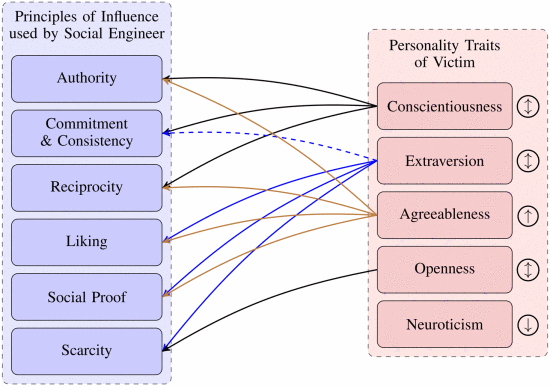
\includegraphics[scale=.55]{FFM.png}
    \caption{Anfälligkeit verschiedener Persönlichkeitseigenschaften durch die Prinzipien der Beeinflussung, welche von Social Engineers verwendet werden (die Färbung der Pfeile ist außer Acht zu lassen; gestrichelte Linien weisen auf eine negative Korrelation hin). Entnommen aus \bcite{7_mdpi}.}
\end{figure}
\FloatBarrier

Gewissenhaftigkeit erhöht die Empfänglichkeit für Autorität, Engagement/Konsistenz und Reziprozität.
Extraversion erhöht die Empfänglichkeit für Sympathie und soziale Anerkennung (soziale Beweise) aufgrund ihrer Verbindung mit Geselligkeit.
Hohe Grade der Verträglichkeit korrelieren mit der Tendenz, anderen zu vertrauen und erhöhen die Anfälligkeit für Social Engineering, da sie anfälliger für Überzeugung und Autorität sind
und mehr Interesse an sozialer Bestätigung, Reziprozität und Sympathie haben.
Offenheit ist mit erhöhter Anfälligkeit für Social Engineering Taktiken verbunden, da sie mit der sozialen Neigung einhergeht, Neues erleben zu wollen.
Neurotizismus ist mit Stress und Angst verbunden, was wiederum die Anfälligkeit gegebenenfalls verringern kann \bcite{psyexploiting,7_mdpi}.

Nach dem DT-Modell haben narzisstische (oder psychopathische) Tendenzen eine Korrelation dazu, den Angreifer einer Social Engineering Attacke zu repräsentieren.
Narzissmus zeichnet sich zumeist aus durch hohe Extraversion und hohen Neurotizismus sowie niedrige Verträglichkeit \bcite{psyexploiting}.

Insgesamt ist also zu sehen, dass nahezu alle Persönlichkeiten auf gewisse Manipulationstechniken ansprechen.
Daher ist also auch nahezu jede Person bei Verwendung eines spezifischen und passenden Prinzips der Beeinflussung manipulierbar.
